\section{Introduction}

We first present (in a very introductory manner) the task of word-alignment and the used tools. In two parts of the evaluation, we first present and evaluate simple word alignment models individually (\Cref{sec:individual}) and then enhanced with new features and combined together using a neural network (\Cref{sec:aggregated}). In both cases, we explore the models' behaviour on Czech-English and German-English datasets.

All of the code is available\footnotehref{https://github.com/zouharvi/LeverageAlign}{github.com/zouharvi/LeverageAlign} open-source.

\subsection{Word Alignment}

Word alignment (also bitext alignment) is a task of matching two groups of words together that are each other's semantic translation. This is, of course, problematic for non-content words, which are specific for the given language, but generally one is able to construct a mapping as in the example in \Cref{fig:alignment_example}. Word alignment usually follows after sentence alignment.  Even though it is called word alignment, it usually operates also on tokens.
% \footnote{Drawn using \href{https://vilda.net/s/slowalign/}{vilda.net/s/slowalign}. More complex word alignment illustrations are available with \href{https://github.com/M4t1ss/SoftAlignments}{github.com/M4t1ss/SoftAlignments}}

\begin{figure*}[h!]
    \center
    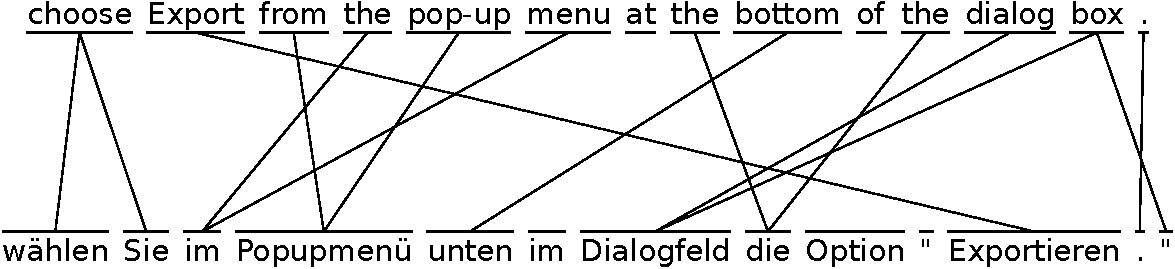
\includegraphics[width=0.75\textwidth]{img/alignment_example.pdf}
    \caption{
        Illustration of English-German word alignment. Source token \textit{choose} is aligned to two target tokens \textit{wählen} and \textit{Sie}, while the target token \textit{Option} is left unaligned. The target article \textit{die} is mistakenly aligned to two unrelated articles \textit{the}.
        \label{fig:alignment_example}
    }
\end{figure*}

Although word alignment found its use mainly in phrase-based machine translation (for generating phrase tables), it is still useful for many other tasks and applications: boosting MT performance \citep{alkhouli2016alignment}, exploring cross-linguistic phenomena \citep{schrader2006does}, computing quality estimation \citep{specia2013quest}, presenting quality estimation \citep{zouhar2020extending} or simply highlighting matching words and phrases in interactive MT (publicly available MT services).

Word alignment output can be formalized as a set containing tuples of source and target words. For output $A$ and gold alignment $G$, precision can be computes as: $ |A \cap G| / |A|$ and recall as $|A \cap G| / |G|$. F score is defined in a standard manner. These evaluation measures are very well described by \citet{mihalcea2003evaluation}.

\subsection{Relevant Work}

The work of \citet{li2019word} is closely related to this article, as it systematically examines the issue of word alignment from NMT and proposes two ways of extracting it: prediction difference and explicit model. They also show that without guided alignment in training, NMT systems perform worse than \fastalign{} baseline.

\subsection{Tools}

For the purposes of this experiment, we need two main tools: IBM model based word aligner and an MT system capable of providing output probabilities and optionally also attention-based word alignment.

\paragraph{\fastalign} \citep{dyer2013simple} is a word aligner based on IBM Alignment Model 2. It does not provide state of the art pre-neural performance but is easy to build with modern toolchains and has low resource requirements (both memory- and computational-wise).

\paragraph{MarianNMT} \citep{junczys2018marian} is a popular (both in academia and in deployment scenarios) actively developed and maintained system for machine translation. It already contains options for producing word alignment and output probabilities.

\subsection{Data}

For training purposes, we make use mostly of the manually annotated parallel corpora of word alignment Czech-English by \citet{marecek_csen_algn_corpus}. We also include German-English Big corpus by \citet{rozis_tilde}, which has not been word-aligned. From this corpus, 1M sentences were sampled randomly. The manually aligned German-English Small corpus by \citet{bicini_ende_algn_corpus} is included for testing. Overview of the corpus sizes is shown in \Cref{tab:corpus_used}.

\begin{table*}[h!]
    \center
    \begin{tabular}{lccccc}
        \toprule
        CS/DE-English & Type & Domain &\hspace{-0.1cm}CS/DE Tokens & EN Tokens & Sentences \\
        \cmidrule{1-6}
        Czech- & aligned & news, legal & 106k & 119k & 5k \\
        German- Small\hspace{-0.2cm} & aligned & legal & 1445 & 1478 & 100 \\
        German- Big & unaligned &tech, news, legal & 23M & 24M & 1M \\
        \bottomrule
    \end{tabular}
    \caption{Used word aligned corpora with their sizes, domains and origin. \label{tab:corpus_used}}
\end{table*}

\subsection{MT Models}

We make use of the MT models made available\footnotehref{https://github.com/browsermt/students}{github.com/browsermt/students} by the \citet{model_csen} and \citet{model_deen}. For both Czech-English and English-German, CPU-optimized student models are used. They are transformer based \citep{vaswani2017transformer} and were created by knowledge distillation, as proposed by \citet{germann-EtAl:2020:WMT}. With WM18 SacreBLEU \citep{sacrebleu}, the models achieve the following BLEU scores: Czech-English (32.6), English-Czech (27.9) and English-German (46.4).